% Options for packages loaded elsewhere
\PassOptionsToPackage{unicode}{hyperref}
\PassOptionsToPackage{hyphens}{url}
\PassOptionsToPackage{dvipsnames,svgnames,x11names}{xcolor}
%
\documentclass[
  letterpaper,
  DIV=11,
  numbers=noendperiod]{scrartcl}

\usepackage{amsmath,amssymb}
\usepackage{iftex}
\ifPDFTeX
  \usepackage[T1]{fontenc}
  \usepackage[utf8]{inputenc}
  \usepackage{textcomp} % provide euro and other symbols
\else % if luatex or xetex
  \usepackage{unicode-math}
  \defaultfontfeatures{Scale=MatchLowercase}
  \defaultfontfeatures[\rmfamily]{Ligatures=TeX,Scale=1}
\fi
\usepackage{lmodern}
\ifPDFTeX\else  
    % xetex/luatex font selection
\fi
% Use upquote if available, for straight quotes in verbatim environments
\IfFileExists{upquote.sty}{\usepackage{upquote}}{}
\IfFileExists{microtype.sty}{% use microtype if available
  \usepackage[]{microtype}
  \UseMicrotypeSet[protrusion]{basicmath} % disable protrusion for tt fonts
}{}
\makeatletter
\@ifundefined{KOMAClassName}{% if non-KOMA class
  \IfFileExists{parskip.sty}{%
    \usepackage{parskip}
  }{% else
    \setlength{\parindent}{0pt}
    \setlength{\parskip}{6pt plus 2pt minus 1pt}}
}{% if KOMA class
  \KOMAoptions{parskip=half}}
\makeatother
\usepackage{xcolor}
\setlength{\emergencystretch}{3em} % prevent overfull lines
\setcounter{secnumdepth}{-\maxdimen} % remove section numbering
% Make \paragraph and \subparagraph free-standing
\ifx\paragraph\undefined\else
  \let\oldparagraph\paragraph
  \renewcommand{\paragraph}[1]{\oldparagraph{#1}\mbox{}}
\fi
\ifx\subparagraph\undefined\else
  \let\oldsubparagraph\subparagraph
  \renewcommand{\subparagraph}[1]{\oldsubparagraph{#1}\mbox{}}
\fi

\usepackage{color}
\usepackage{fancyvrb}
\newcommand{\VerbBar}{|}
\newcommand{\VERB}{\Verb[commandchars=\\\{\}]}
\DefineVerbatimEnvironment{Highlighting}{Verbatim}{commandchars=\\\{\}}
% Add ',fontsize=\small' for more characters per line
\usepackage{framed}
\definecolor{shadecolor}{RGB}{241,243,245}
\newenvironment{Shaded}{\begin{snugshade}}{\end{snugshade}}
\newcommand{\AlertTok}[1]{\textcolor[rgb]{0.68,0.00,0.00}{#1}}
\newcommand{\AnnotationTok}[1]{\textcolor[rgb]{0.37,0.37,0.37}{#1}}
\newcommand{\AttributeTok}[1]{\textcolor[rgb]{0.40,0.45,0.13}{#1}}
\newcommand{\BaseNTok}[1]{\textcolor[rgb]{0.68,0.00,0.00}{#1}}
\newcommand{\BuiltInTok}[1]{\textcolor[rgb]{0.00,0.23,0.31}{#1}}
\newcommand{\CharTok}[1]{\textcolor[rgb]{0.13,0.47,0.30}{#1}}
\newcommand{\CommentTok}[1]{\textcolor[rgb]{0.37,0.37,0.37}{#1}}
\newcommand{\CommentVarTok}[1]{\textcolor[rgb]{0.37,0.37,0.37}{\textit{#1}}}
\newcommand{\ConstantTok}[1]{\textcolor[rgb]{0.56,0.35,0.01}{#1}}
\newcommand{\ControlFlowTok}[1]{\textcolor[rgb]{0.00,0.23,0.31}{#1}}
\newcommand{\DataTypeTok}[1]{\textcolor[rgb]{0.68,0.00,0.00}{#1}}
\newcommand{\DecValTok}[1]{\textcolor[rgb]{0.68,0.00,0.00}{#1}}
\newcommand{\DocumentationTok}[1]{\textcolor[rgb]{0.37,0.37,0.37}{\textit{#1}}}
\newcommand{\ErrorTok}[1]{\textcolor[rgb]{0.68,0.00,0.00}{#1}}
\newcommand{\ExtensionTok}[1]{\textcolor[rgb]{0.00,0.23,0.31}{#1}}
\newcommand{\FloatTok}[1]{\textcolor[rgb]{0.68,0.00,0.00}{#1}}
\newcommand{\FunctionTok}[1]{\textcolor[rgb]{0.28,0.35,0.67}{#1}}
\newcommand{\ImportTok}[1]{\textcolor[rgb]{0.00,0.46,0.62}{#1}}
\newcommand{\InformationTok}[1]{\textcolor[rgb]{0.37,0.37,0.37}{#1}}
\newcommand{\KeywordTok}[1]{\textcolor[rgb]{0.00,0.23,0.31}{#1}}
\newcommand{\NormalTok}[1]{\textcolor[rgb]{0.00,0.23,0.31}{#1}}
\newcommand{\OperatorTok}[1]{\textcolor[rgb]{0.37,0.37,0.37}{#1}}
\newcommand{\OtherTok}[1]{\textcolor[rgb]{0.00,0.23,0.31}{#1}}
\newcommand{\PreprocessorTok}[1]{\textcolor[rgb]{0.68,0.00,0.00}{#1}}
\newcommand{\RegionMarkerTok}[1]{\textcolor[rgb]{0.00,0.23,0.31}{#1}}
\newcommand{\SpecialCharTok}[1]{\textcolor[rgb]{0.37,0.37,0.37}{#1}}
\newcommand{\SpecialStringTok}[1]{\textcolor[rgb]{0.13,0.47,0.30}{#1}}
\newcommand{\StringTok}[1]{\textcolor[rgb]{0.13,0.47,0.30}{#1}}
\newcommand{\VariableTok}[1]{\textcolor[rgb]{0.07,0.07,0.07}{#1}}
\newcommand{\VerbatimStringTok}[1]{\textcolor[rgb]{0.13,0.47,0.30}{#1}}
\newcommand{\WarningTok}[1]{\textcolor[rgb]{0.37,0.37,0.37}{\textit{#1}}}

\providecommand{\tightlist}{%
  \setlength{\itemsep}{0pt}\setlength{\parskip}{0pt}}\usepackage{longtable,booktabs,array}
\usepackage{calc} % for calculating minipage widths
% Correct order of tables after \paragraph or \subparagraph
\usepackage{etoolbox}
\makeatletter
\patchcmd\longtable{\par}{\if@noskipsec\mbox{}\fi\par}{}{}
\makeatother
% Allow footnotes in longtable head/foot
\IfFileExists{footnotehyper.sty}{\usepackage{footnotehyper}}{\usepackage{footnote}}
\makesavenoteenv{longtable}
\usepackage{graphicx}
\makeatletter
\def\maxwidth{\ifdim\Gin@nat@width>\linewidth\linewidth\else\Gin@nat@width\fi}
\def\maxheight{\ifdim\Gin@nat@height>\textheight\textheight\else\Gin@nat@height\fi}
\makeatother
% Scale images if necessary, so that they will not overflow the page
% margins by default, and it is still possible to overwrite the defaults
% using explicit options in \includegraphics[width, height, ...]{}
\setkeys{Gin}{width=\maxwidth,height=\maxheight,keepaspectratio}
% Set default figure placement to htbp
\makeatletter
\def\fps@figure{htbp}
\makeatother

\KOMAoption{captions}{tableheading}
\makeatletter
\makeatother
\makeatletter
\makeatother
\makeatletter
\@ifpackageloaded{caption}{}{\usepackage{caption}}
\AtBeginDocument{%
\ifdefined\contentsname
  \renewcommand*\contentsname{Table of contents}
\else
  \newcommand\contentsname{Table of contents}
\fi
\ifdefined\listfigurename
  \renewcommand*\listfigurename{List of Figures}
\else
  \newcommand\listfigurename{List of Figures}
\fi
\ifdefined\listtablename
  \renewcommand*\listtablename{List of Tables}
\else
  \newcommand\listtablename{List of Tables}
\fi
\ifdefined\figurename
  \renewcommand*\figurename{Figure}
\else
  \newcommand\figurename{Figure}
\fi
\ifdefined\tablename
  \renewcommand*\tablename{Table}
\else
  \newcommand\tablename{Table}
\fi
}
\@ifpackageloaded{float}{}{\usepackage{float}}
\floatstyle{ruled}
\@ifundefined{c@chapter}{\newfloat{codelisting}{h}{lop}}{\newfloat{codelisting}{h}{lop}[chapter]}
\floatname{codelisting}{Listing}
\newcommand*\listoflistings{\listof{codelisting}{List of Listings}}
\makeatother
\makeatletter
\@ifpackageloaded{caption}{}{\usepackage{caption}}
\@ifpackageloaded{subcaption}{}{\usepackage{subcaption}}
\makeatother
\makeatletter
\@ifpackageloaded{tcolorbox}{}{\usepackage[skins,breakable]{tcolorbox}}
\makeatother
\makeatletter
\@ifundefined{shadecolor}{\definecolor{shadecolor}{rgb}{.97, .97, .97}}
\makeatother
\makeatletter
\makeatother
\makeatletter
\makeatother
\ifLuaTeX
  \usepackage{selnolig}  % disable illegal ligatures
\fi
\IfFileExists{bookmark.sty}{\usepackage{bookmark}}{\usepackage{hyperref}}
\IfFileExists{xurl.sty}{\usepackage{xurl}}{} % add URL line breaks if available
\urlstyle{same} % disable monospaced font for URLs
\hypersetup{
  pdftitle={Analyse de l'impact du genre sur la saillance des thématiques politiques féminines dans le discours des politicien(ne)s},
  pdfauthor={Olivia Saffioti},
  colorlinks=true,
  linkcolor={blue},
  filecolor={Maroon},
  citecolor={Blue},
  urlcolor={Blue},
  pdfcreator={LaTeX via pandoc}}

\title{Analyse de l'impact du genre sur la saillance des thématiques
politiques féminines dans le discours des politicien(ne)s}
\author{Olivia Saffioti}
\date{}

\begin{document}
\maketitle
\ifdefined\Shaded\renewenvironment{Shaded}{\begin{tcolorbox}[boxrule=0pt, enhanced, breakable, borderline west={3pt}{0pt}{shadecolor}, frame hidden, interior hidden, sharp corners]}{\end{tcolorbox}}\fi

\hypertarget{introduction}{%
\subsection{Introduction}\label{introduction}}

Selon la théorie de la construction sociale du genre, les électeurs
évalueraient les politicien(ne)s en fonction des stéréotypes de genre.
Si les politicien(ne)s n'adaptent par leur stratégie marketing aux
stéréotypes, ils risqueraient un blacklash, soit, des évaluations
négatives de la part des électeurs (Rudman et Fairchild 2004; Coyle
2009, cités dans Grebelsky-Lichtman et Katz 2019). Ainsi les femmes et
les hommes politiques, n'useraient pas des mêmes stratégies marketing
afin de convaincre l'électorat. En effet,~les femmes et les hommes
répondraient souvent aux stéréotypes induits par le rôle attribué à
chaque sexe dans la société. Ils conforteraient ainsi la vision des
électeurs (Fox 1997). Cela incluerait l'image, les caractéristiques
personnelles, les thèmes de campagne, et l'utilisation d'enjeux
politiques spécifiques (Fox 1997). À titre d'exemple, les femmes
politiques seraient perçues par l'électorat comme plus efficaces dans
les domaines de l'éducation, de la santé, de l'environnement, des arts,
de la protection des consommateurs, ou encore dans l'aide à apporter aux
pauvres (Alexander and Andersen 1993; Koch 2000; McDermott 1998, cités
dans Fox et Oxley 2003). À l'inverse, les hommes politiques seraient
considérés comme plus compétents pour résoudre des crises militaires ou
de police, des problèmes d'ordre économique, ou encore des enjeux liés
au commerce. Ils seraient également identifiés comme plus légitimes pour
s'occuper du contrôle de la criminalité ou encore de l'agriculture
(Alexander and Andersen 1993; Koch 2000; McDermott 1998, cités dans Fox
et Oxley 2003). En revanche, ces études ont surtout été menée au sein du
contexte étasunien, et nous n'avons trouvé que peu de recherches qui
visent les stratégies des femmes et des hommes politiques lors des
débats électoraux. Il semble ainsi pertinent d'étudier si les femmes
politiques insistent davantage sur les thématiques «~féminines~»
(éducation, etc.) par rapport à leurs homologues masculins, dans un
débat électoral qui n'est pas étasunien . C'est pourquoi, nous avons
décidé d'étudier le débat électoral français opposant Marine Le Pen et
Emmanuel Macron en 2017. Nous avons choisi ce débat car sa
retranscription était facile d'accès. De plus, sélectionner un débat qui
s'était produit après 2019 aurait biaisé nos résultats. En effet, la
pandémie de Covid-19 demeurait un sujet très discuté par les politiciens
durant les campagnes suivant 2019. Ce contexte temporel ne nous aurait
pas permis de vérifier si les femmes politiques parlaient davantage de
la santé que les hommes. À travers ce débat nous vérifierons si madame
Le Pen a plus insisté sur les enjeux de l'éducation, de la famille, de
l'État Providence et de la santé que monsieur Macron. Cela nous
permettra de vérifier si les postulats de la théorie de la construction
sociale du genre sont applicables à d'autres contextes. Pour ce faire,
nous utiliserons la base de données portant sur le débat électoral entre
Emmanuel Macron et Marine Le Pen de 2017 (Fréchet 2024). Puis, nous la
nettoierons. Ensuite, nous élaborerons un dictionnaire. À partir de ce
dernier, nous analyserons notre base de données. Afin de mieux
visualiser et comprendre nos résultats, nous élaborerons un graphique.~

\hypertarget{donnuxe9es-et-muxe9thode}{%
\subsection{Données et méthode}\label{donnuxe9es-et-muxe9thode}}

Afin de mener notre recherche, nous avons utilisé la base de données
portant sur le débat présidentiel entre Marine Le Pen et Emmanuel Macron
de 2017. Cette base de données a été créé par monsieur Nadjim Fréchet,
doctorant à l'Université de Montréal, et spécialiste en analyse
quantitative. Elle contient plusieurs variables : une variable ``text''
exposant le texte du débat, une variable ``speaker'' exposant le nom des
intervenants du débat, une variable ``party'' indiquant le parti
d'appartenance ou la profession des intervenants, une variable
``speaker\_turn'' indiquant dans quel ordre les intervenants parlent,
une variable ``id'' indiquant à quel tour des élections présidentielles
correspond le débat, une variable ``year'' indiquant l'année du débat,
une variable ``date'' indiquant la date précise du débat (jour, mois,
année), et une variable ``country'' exposant le pays dans lequel le
débat a eu lieu. Dans cette base de donnée, deux variables nous ont
interessées : la variable ``text'' et la variable ``speaker''. Afin
d'analyser cette base de données, nous l'avons tout d'abord importé sur
Rstudio afin de la nettoyer et d'opérer une analyse de dictionnaire.

Dans un premier temps, nous avons créé notre dictionnaire afin de
pouvoir analyser la fréquence de certains mots dans le discours des
candidats. Personnaliser notre dictionnaire nous a permis de faire une
analyse qui corrélait avec le contexte (les thématiques évoquées dans le
débat) et notre sujet de recherche. Nous avons pu prendre en compte des
mots spécifiques tels que ``protection sociale'' ou ``quotient''. Les
mots du dictionnaire sont reliés aux thématiques ``féminines'' de
l'éducation, de la santé, de la famille, et de l'État providence (lutte
contre la pauvreté, etc.). Afin de créer le dictionnaire, nous avons
mobilisé la fonction ``list( )'', et la fonction ``dictionnary( )'' du
package quanteda.

Puis, nous avons nettoyé notre base de données : nous avons retiré les
ponctuations du texte et converti le texte en minuscules. Cela nous
permettait par la suite de faciliter notre analyse de dictionnaire.
Effectivement, un mot présent dans notre dictionnaire en minuscules
risquerait de ne pas être détecté lors de notre analyse de dictionnaire
si le texte comprend des majuscules. Les virgules pourraient également
perturber l'analyse de dictionnaire. C'est pourquoi, nous avons mobilisé
les fonctions ``tolower( )'' et ``gsub( )''. Nous avons disposé notre
texte nettoyé dans une nouvelle colonne nommée ``text\_clean''. Ensuite,
nous avons sélectionner les variables que nous voulions conserver dans
notre base de données, afin de retirer les variables inutiles. Nous
avons décidé de conserver les variables ``text\_clean'' et ``speaker''.
Dans la variable ``speaker'' nous avons conservé uniquement deux
speakers (deux catégories) : ``Le Pen'' et ``Macron''. Nous avons choisi
de les conserver car nous nous centrons uniquement sur ces deux
candidats dans le cadre de notre étude. Pour cela, nous avons utilisé
les fonctions ``select( )'' et ``filter( )'' du package dplyr, présent
dans le package tidyverse. Ensuite, nous avons procédé à notre analyse
de dictionnaire, et transféré les résultats dans une nouvelle base de
données intitulée ``debat\_macron\_lepen\_resultat''. Pour ce faire,
nous avons mobilisé la fonction ``run\_dictionary( )'' issue du package
clessnverse, la fonction ``bind\_cols( )'' et la fonction ``select( )''
provenants du package dplyr. '' run\_dictionary( )'' nous a permis de
``rouler'' notre dictionnaire afin qu'il relève les mots dans le texte.
La fonction bind\_cols a permis de conserver les colonnes présentes dans
la base de données ``debat\_macron\_lepen'', dans notre nouvelle base de
données ``debat\_macron\_lepen\_resultat''. La fonction select( ) nous a
permis de sélectionner les colonnes que nous ne voulions pas garder dans
``debat\_macron\_lepen\_resultat'' (ici, nous n'avons pas conservé la
variable ``doc\_id'').

Afin de pouvoir conceptualiser notre grahique, nous avons converti notre
base de données en format long. Pour ce faire, nous avons dans un
premier temps créé un tableau où les résultats de notre analyse de
dictionnaire ont été résumés. Ce tableau se nomme
``donnees\_graphique'', et a été créé grâce aux fonctions group\_by( )
et summarise( ) du package dplyr. ``group\_by ( )'' nous a permis de
regrouper les données en fonction des locuteurs. ``summarise ( )'' nous
a permis de résumer les données des catégories de notre dictionnaire
(santé, éducation, état\_providence et famille). Puis, nous avons
converti la base de données ``donnees\_graphique'' en format long grâce
à la fonction ``pivot\_longer( )'' du package tidyr. Cette nouvelle base
de données a été intitulée ``donnees\_graphique\_format\_long''. Nous
avons finalement élaboré notre graphique à partir de la base de données
convertie au format long.

\hypertarget{ruxe9sultats}{%
\subsection{Résultats}\label{ruxe9sultats}}

\begin{figure}

{\centering 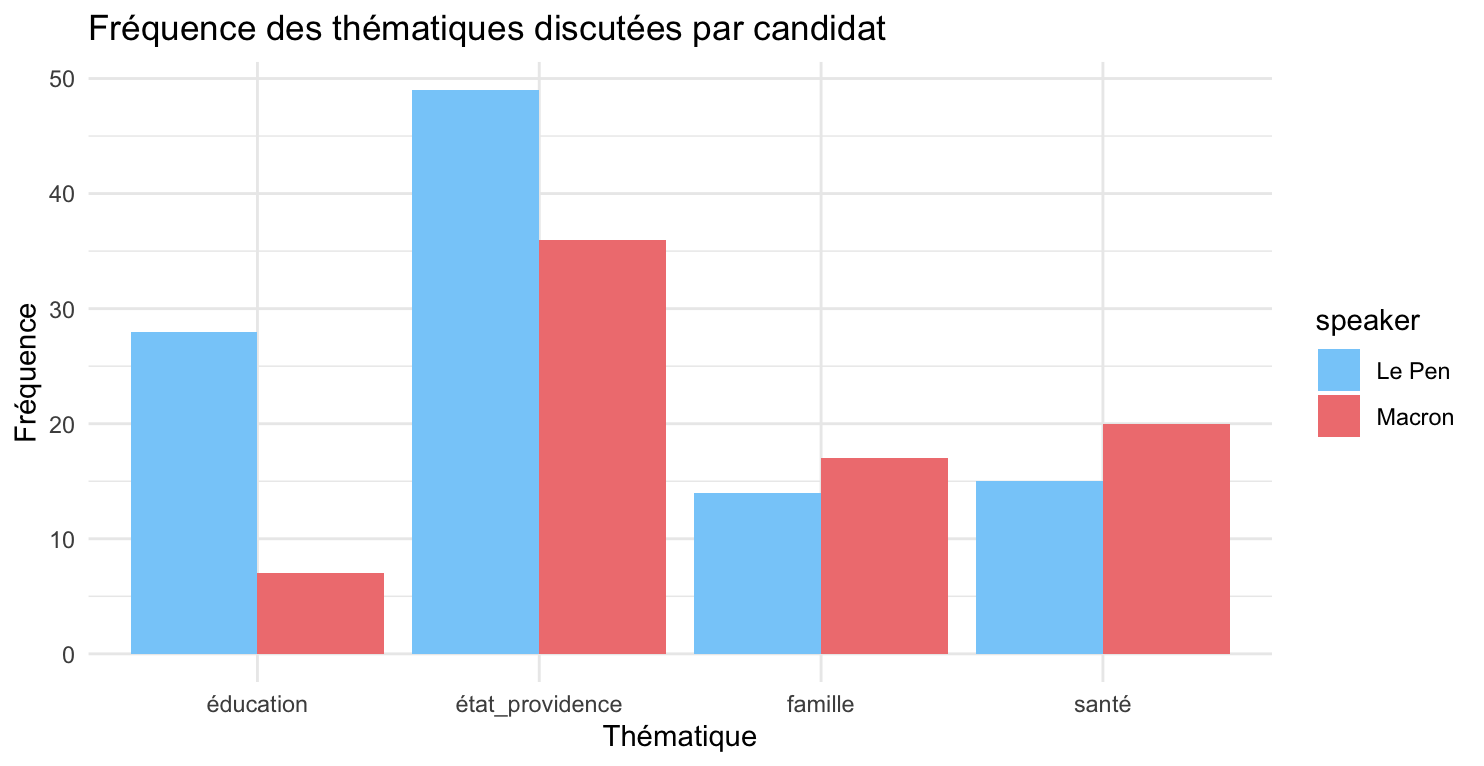
\includegraphics{/Users/oliviasaffioti/Desktop/fas_1001_Saffioti/_tp/TP3/Graphique-TP3.png}

}

\caption{Graphique}

\end{figure}

Les résultats que nous avons obtenu indiquent que Marine Le Pen et
Emmanuel Macron n'auraient pas insisté de la même manière sur les enjeux
de la santé, de la famille, de l'État providence et de l'éducation. En
effet, 49 mots liés à l'État providence ont été relevés dans le discours
de Marine Le Pen. Comparativement, 36 mots ont été relevés dans le
discours d'Emmanuel Macron. 13 mots de plus ont été relevés pour Marine
Le Pen par rapport à Emmanuel Macron. Bien que les deux candidats aient
beaucoup insisté sur cette thématique, il semblerait que madame Le Pen
ait plus insisté sur les éléments liés à l'état-providence que monsieur
Macron. De plus, 28 mots liés à l'éducation ont été soulevés dans les
paroles de Le Pen, contre seulement 7 pour Macron. Il y a donc un écart
important de 21 mots entre Le Pen et Macron. Madame Le Pen aurait donc
plus insisté sur la thématique de l'éducation que monsieur Macron. En
revanche, concernant la thématique de la famille, l'écart entre les deux
candidats n'est pas élevé : il est seulement de 3 mots. En effet, 14
mots ont été relevés dans le discours de madame Le Pen contre 17 pour
monsieur Macron. Il semblerait donc que les deux candidats aient insisté
de manière à peu près équivalente sur la thématique de la famille.
Enfin, concernant la thématique de la santé, 15 mots ont été relevés
dans le cas de madame Le Pen et 20 dans le cas de monsieur Macron. Là
encore, l'écart n'est pas important entre Le Pen et Macron (il est
seulement de 5 mots). Il semblerait que monsieur Macron et madame Lepen
aient insisté de manière à peu près équivalente sur la thématique de la
santé.

Dans l'ensemble, plus de mots liés à la famille et à la santé ont été
relevés pour Emmanuel Macron. En revanche, l'écart avec madame Le Pen
n'est pas élevé. Les écarts de mots pour ces deux thématiques ne sont
pas significatifs : ils ne démontrent pas que Macron aurait plus insisté
que Lepen sur ces deux thématiques. En revanche, l'écart entre Macron et
Lepen est plus prononcé concernant la thématique de l'éducation et de
l'état providence. Lepen et Macron ont insisté de manière équivalente
sur la santé et la famille, mais Lepen a plus insisté que Macron sur
l'État providence et l'éducation. Par conséquent, Marine Le Pen semble,
généralement, avoir davantage insisté sur les thématiques ``féminines''
par rapport à Emmanuel Macron. Donc, il semblerait que, dans le cas du
débat présidentiel entre Emmanuel Macron et Marine Lepen de 2017, le
postulat selon lequel les femmes politiques insisteraient davantage sur
les thématiques ``féminines'' (santé, éducation, etc.) soit validé.

\hypertarget{conclusion}{%
\subsection{Conclusion}\label{conclusion}}

En somme, nous avons étudié le débat présidentiel de 2017 opposant
Emmanuel Macron à Marine Lepen afin de vérifier si madame Lepen
insistait davantage sur les thématiques ``féminines'' que monsieur
Macron. Les résultats issus de notre analyse de dictionnaire ont montré
que madame Lepen insistait davantage sur les thématiques de
l'État\_providence et de l'éducation. De plus, Macron et Lepen
insistaient avec une fréquence de mots quasi-identique sur la famille et
la santé. Nous avons conclu que, généralement, Marine Lepen avait plus
insisté sur les thématiques féminines qu'Emmanuel Macron dans le cadre
de ce débat électoral. En revanche, notre recherche a une faible
validité externe : il aurait fallu étudier plusieurs débats électoraux
de Marine Lepen pour savoir si la candidate a insisté sur ces
thématiques dans le cadre d'autres débats électoraux. De surcroît, il
aurait été pertinent d'étudier des débats électoraux incluant d'autres
femmes issues de partis politiques différents. Cela aurait permis de
contrôler pour le parti d'appartenance, et donc de vérifier si
l'insistance sur les enjeux féminins dépend de la ligne idéologique du
parti politique des politicien(ne)s (et non du genre).

\hypertarget{bibliographie}{%
\subsection{Bibliographie}\label{bibliographie}}

Fox, Richard Logan. 1997. \emph{Gender Dynamics in Congressional
Elections.} Thousand Oaks: Éditions SAGE.
https://books.google.ca/books?hl=en\&lr=\&id=x2w1BfJwRkAC\&oi=fnd\&pg=PR13\&dq=gender+women+elections\&ots=8RGQYfimmw\&sig=Uo31w\_YYAhrRtOEKSyA6ABiEeWw\#v=onepage\&q=gender\%20women\%20elections\&f=false

Fox, Richard L., et Zoe M. Oxley. 2003. ``Gender Stereotyping in State
Executive Elections: Candidate Selection and Success''. \emph{The
Journal of Politics} 65 (3): 833-50.
https://doi.org/10.1111/1468-2508.00214.

Fréchet, Nadjim. 2024. \emph{Base de données portant sur le débat
électoral entre Emmanuel Macron et Marine Le Pen de 2017}.

Grebelsky-Lichtman, Tsfira, Roy Katz. 2019. '' When a man debates a
woman : Trump vs.Clinton in the first mixed gender presidential debate
``. \emph{Revue Journal of Gender Studies} 28 (6): 699-719.
https://www.tandfonline.com/doi/full/10.1080/09589236.2019.1566890

\hypertarget{annexe}{%
\subsection{Annexe}\label{annexe}}

\begin{Shaded}
\begin{Highlighting}[]
\CommentTok{\# Codes de monsieur Nadjim Fréchet afin de convertir le texte pdf en base de données csv : }

\DocumentationTok{\#\# Libraries}

\FunctionTok{library}\NormalTok{(pdftools)}
\end{Highlighting}
\end{Shaded}

\begin{verbatim}
Using poppler version 23.04.0
\end{verbatim}

\begin{Shaded}
\begin{Highlighting}[]
\FunctionTok{library}\NormalTok{(tidyverse)}
\end{Highlighting}
\end{Shaded}

\begin{verbatim}
-- Attaching core tidyverse packages ------------------------ tidyverse 2.0.0 --
v dplyr     1.1.4     v readr     2.1.5
v forcats   1.0.0     v stringr   1.5.1
v ggplot2   3.4.4     v tibble    3.2.1
v lubridate 1.9.3     v tidyr     1.3.0
v purrr     1.0.2     
\end{verbatim}

\begin{verbatim}
-- Conflicts ------------------------------------------ tidyverse_conflicts() --
x dplyr::filter() masks stats::filter()
x dplyr::lag()    masks stats::lag()
i Use the conflicted package (<http://conflicted.r-lib.org/>) to force all conflicts to become errors
\end{verbatim}

\begin{Shaded}
\begin{Highlighting}[]
\FunctionTok{library}\NormalTok{(lubridate)}

\DocumentationTok{\#\# Data}

\NormalTok{text\_1 }\OtherTok{\textless{}{-}} \FunctionTok{suppressMessages}\NormalTok{(pdftools}\SpecialCharTok{::}\FunctionTok{pdf\_text}\NormalTok{(}\StringTok{"/Users/oliviasaffioti/Desktop/fas\_1001\_Saffioti/\_tp/TP3/macron\_vs\_lepen.pdf"}\NormalTok{))}

\DocumentationTok{\#\# Settings}

\NormalTok{split\_vector }\OtherTok{\textless{}{-}} \FunctionTok{paste0}\NormalTok{(}\FunctionTok{c}\NormalTok{(}\StringTok{"Mme Le Pen :"}\NormalTok{, }\StringTok{"Mme Saint{-}Cricq :"}\NormalTok{, }\StringTok{"M. Jakubyszyn :"}\NormalTok{, }\StringTok{"M. Macron :"}\NormalTok{, }\StringTok{"https"}\NormalTok{), }\AttributeTok{collapse =} \StringTok{"|"}\NormalTok{)}


\DocumentationTok{\#\# Nettoyage de code}

\DocumentationTok{\#\# Chercher les nom des personnes concernéés dans le débat}

\NormalTok{speaker\_names }\OtherTok{\textless{}{-}} \FunctionTok{data.frame}\NormalTok{(}\AttributeTok{text =} \FunctionTok{paste0}\NormalTok{(text\_1, }\AttributeTok{collapse =} \StringTok{" "}\NormalTok{)) }\SpecialCharTok{|\textgreater{}}
  \FunctionTok{mutate}\NormalTok{(}\AttributeTok{text =} \FunctionTok{str\_squish}\NormalTok{(}\FunctionTok{str\_replace\_all}\NormalTok{(text, }\FunctionTok{c}\NormalTok{(}\StringTok{"[:punct:]C2[:punct:]AB"}  \OtherTok{=} \StringTok{""}\NormalTok{,}
                                                   \StringTok{"[:punct:]C2[:punct:]BB"}  \OtherTok{=} \StringTok{""}\NormalTok{))),}
         \AttributeTok{text =} \FunctionTok{str\_replace\_all}\NormalTok{(text, }\FunctionTok{c}\NormalTok{(}\StringTok{"Emmanuel Macron :"}       \OtherTok{=} \StringTok{"M. Macron :"}\NormalTok{,}
                                        \StringTok{"Marine Le Pen :"}         \OtherTok{=} \StringTok{"Mme Le Pen :"}\NormalTok{,}
                                        \StringTok{"Christophe Jakubyszyn :"} \OtherTok{=} \StringTok{"M. Jakubyszyn :"}\NormalTok{,}
                                        \StringTok{"Nathalie Saint{-}Cricq :"}  \OtherTok{=} \StringTok{"Mme Saint{-}Cricq :"}\NormalTok{)),}
         \AttributeTok{speaker =} \FunctionTok{str\_extract\_all}\NormalTok{(text, split\_vector)) }\SpecialCharTok{|\textgreater{}} 
  \FunctionTok{select}\NormalTok{(}\SpecialCharTok{{-}}\NormalTok{text) }\SpecialCharTok{|\textgreater{}} 
  \FunctionTok{unnest}\NormalTok{(speaker) }\SpecialCharTok{|\textgreater{}} 
  \FunctionTok{slice}\NormalTok{(}\SpecialCharTok{{-}}\DecValTok{805}\NormalTok{)}
  
\DocumentationTok{\#\# Données de prises de parole (text data)}

\NormalTok{text\_data }\OtherTok{\textless{}{-}} \FunctionTok{data.frame}\NormalTok{(}\AttributeTok{text =} \FunctionTok{paste0}\NormalTok{(text\_1, }\AttributeTok{collapse =} \StringTok{" "}\NormalTok{)) }\SpecialCharTok{|\textgreater{}} 
    \FunctionTok{mutate}\NormalTok{(}\AttributeTok{text =} \FunctionTok{str\_squish}\NormalTok{(}\FunctionTok{str\_replace\_all}\NormalTok{(text, }\FunctionTok{c}\NormalTok{(}\StringTok{"[:punct:]C2[:punct:]AB"}  \OtherTok{=} \StringTok{""}\NormalTok{,}
                                                     \StringTok{"[:punct:]C2[:punct:]BB"}  \OtherTok{=} \StringTok{""}\NormalTok{))),}
           \AttributeTok{text =} \FunctionTok{str\_replace\_all}\NormalTok{(text, }\FunctionTok{c}\NormalTok{(}\StringTok{"Emmanuel Macron :"}       \OtherTok{=} \StringTok{"M. Macron :"}\NormalTok{,}
                                          \StringTok{"Marine Le Pen :"}         \OtherTok{=} \StringTok{"Mme Le Pen :"}\NormalTok{,}
                                          \StringTok{"Christophe Jakubyszyn :"} \OtherTok{=} \StringTok{"M. Jakubyszyn :"}\NormalTok{,}
                                          \StringTok{"Nathalie Saint{-}Cricq :"}  \OtherTok{=} \StringTok{"Mme Saint{-}Cricq :"}\NormalTok{)),}
           \AttributeTok{text =} \FunctionTok{str\_split}\NormalTok{(text, split\_vector)) }\SpecialCharTok{|\textgreater{}}
  \FunctionTok{unnest}\NormalTok{(text) }\SpecialCharTok{|\textgreater{}} 
  \FunctionTok{slice}\NormalTok{(}\SpecialCharTok{{-}}\FunctionTok{c}\NormalTok{(}\DecValTok{1}\NormalTok{,}\DecValTok{806}\NormalTok{)) }

\DocumentationTok{\#\# Fusion des deux variables clés et création de la base de données finale}

\NormalTok{Data\_debate\_2017 }\OtherTok{\textless{}{-}} \FunctionTok{bind\_cols}\NormalTok{(speaker\_names, text\_data) }\SpecialCharTok{|\textgreater{}} 
  \DocumentationTok{\#\# Creation de variables et nettoyage \#\#}
  \FunctionTok{mutate}\NormalTok{(}\AttributeTok{year         =} \DecValTok{2017}\NormalTok{, }
         \AttributeTok{date         =} \FunctionTok{ymd}\NormalTok{(}\StringTok{"2017{-}05{-}03"}\NormalTok{), }
         \AttributeTok{country      =} \StringTok{"France"}\NormalTok{, }
         \AttributeTok{id           =} \StringTok{"Débat présidentiel 2017 second{-}tour"}\NormalTok{,}
         \AttributeTok{speaker\_turn =} \DecValTok{1}\SpecialCharTok{:}\DecValTok{804}\NormalTok{,}
         \AttributeTok{speaker =} \FunctionTok{str\_squish}\NormalTok{(}\FunctionTok{str\_replace\_all}\NormalTok{(speaker, }\FunctionTok{c}\NormalTok{(}\StringTok{"Mme"} \OtherTok{=} \StringTok{""}\NormalTok{,}
                                                         \StringTok{"\^{}M."} \OtherTok{=} \StringTok{""}\NormalTok{,}
                                                         \StringTok{":"}   \OtherTok{=} \StringTok{""}\NormalTok{))),}
         \AttributeTok{party =} \FunctionTok{case\_when}\NormalTok{(speaker }\SpecialCharTok{==} \StringTok{"Le Pen"} \SpecialCharTok{\textasciitilde{}} \StringTok{"Rassemblement national"}\NormalTok{,}
\NormalTok{                           speaker }\SpecialCharTok{==} \StringTok{"Macron"} \SpecialCharTok{\textasciitilde{}} \StringTok{"Renaissance"}\NormalTok{,}
                           \AttributeTok{.default =} \StringTok{"Journaliste"}\NormalTok{)) }\SpecialCharTok{|\textgreater{}} 
  \FunctionTok{select}\NormalTok{(id, year, date, country, speaker, speaker\_turn, party, text)}

\DocumentationTok{\#\#Sauvegarde des données}

\FunctionTok{write\_csv}\NormalTok{(Data\_debate\_2017, }\StringTok{"/Users/oliviasaffioti/Desktop/fas\_1001\_Saffioti/\_tp/TP3/debat\_macron\_lepen.csv"}\NormalTok{)}
\end{Highlighting}
\end{Shaded}

\begin{Shaded}
\begin{Highlighting}[]
\CommentTok{\# Faire notre recherche avec une analyse de dictionnaire}

\DocumentationTok{\#\#Importer la base de données : }

\FunctionTok{setwd}\NormalTok{(}\StringTok{"/Users/oliviasaffioti/Desktop/fas\_1001\_Saffioti/\_tp/TP3"}\NormalTok{)}
\FunctionTok{getwd}\NormalTok{()}
\end{Highlighting}
\end{Shaded}

\begin{verbatim}
[1] "/Users/oliviasaffioti/Desktop/fas_1001_Saffioti/_tp/TP3"
\end{verbatim}

\begin{Shaded}
\begin{Highlighting}[]
\NormalTok{debat\_macron\_lepen }\OtherTok{\textless{}{-}} \FunctionTok{read.csv}\NormalTok{(}\StringTok{"debat\_macron\_lepen.csv"}\NormalTok{)}

\DocumentationTok{\#\# Libraries :}

\FunctionTok{library}\NormalTok{(quanteda)}
\end{Highlighting}
\end{Shaded}

\begin{verbatim}
Package version: 3.3.1
Unicode version: 14.0
ICU version: 71.1
\end{verbatim}

\begin{verbatim}
Parallel computing: 8 of 8 threads used.
\end{verbatim}

\begin{verbatim}
See https://quanteda.io for tutorials and examples.
\end{verbatim}

\begin{Shaded}
\begin{Highlighting}[]
\FunctionTok{library}\NormalTok{(clessnverse)}
\end{Highlighting}
\end{Shaded}

\begin{verbatim}
DISCLAIMER: As of July 2023, `clessnverse` is no longer under active development.
To avoid breaking dependencies, the package remains available "as is" with no warranty of any kind.
\end{verbatim}

\begin{Shaded}
\begin{Highlighting}[]
\FunctionTok{library}\NormalTok{(tidyverse)}

\DocumentationTok{\#\# Création du dictionnaire : }

\NormalTok{Dictionnaire\_combiné }\OtherTok{\textless{}{-}} \FunctionTok{list}\NormalTok{ (Santé }\OtherTok{=} \FunctionTok{c}\NormalTok{(}\StringTok{"santé"}\NormalTok{, }\StringTok{"médecin"}\NormalTok{, }\StringTok{"hôpital"}\NormalTok{, }\StringTok{"maladie"}\NormalTok{, }\StringTok{"patient"}\NormalTok{, }\StringTok{"soins"}\NormalTok{, }\StringTok{"médecins"}\NormalTok{, }\StringTok{"assurance maladie"}\NormalTok{, }\StringTok{"patients"}\NormalTok{, }\StringTok{"malades"}\NormalTok{, }\StringTok{"médicaments"}\NormalTok{, }\StringTok{"aide médicale"}\NormalTok{, }\StringTok{"visites médicales"}\NormalTok{, }\StringTok{"visite médicale"}\NormalTok{), É}\AttributeTok{ducation =} \FunctionTok{c}\NormalTok{(}\StringTok{"collège"}\NormalTok{, }\StringTok{"enseignement"}\NormalTok{, }\StringTok{"élèves"}\NormalTok{, }\StringTok{"classe"}\NormalTok{, }\StringTok{"classes"}\NormalTok{, }\StringTok{"diplôme"}\NormalTok{, }\StringTok{"diplômes"}\NormalTok{, }\StringTok{"lycée"}\NormalTok{, }\StringTok{"université"}\NormalTok{, }\StringTok{"universités"}\NormalTok{, }\StringTok{"universitaire"}\NormalTok{, }\StringTok{"universitaires"}\NormalTok{, }\StringTok{"formation"}\NormalTok{, }\StringTok{"formations"}\NormalTok{, }\StringTok{"apprentissage"}\NormalTok{, }\StringTok{"filière"}\NormalTok{, }\StringTok{"filières"}\NormalTok{, }\StringTok{"professionnelle"}\NormalTok{, }\StringTok{"professionnelles"}\NormalTok{, }\StringTok{"école"}\NormalTok{), É}\AttributeTok{tat\_providence =} \FunctionTok{c}\NormalTok{(}\StringTok{"retraite"}\NormalTok{, }\StringTok{"protection sociale"}\NormalTok{, }\StringTok{"protections sociales"}\NormalTok{, }\StringTok{"salariés"}\NormalTok{, }\StringTok{"chômage"}\NormalTok{, }\StringTok{"chômeurs"}\NormalTok{, }\StringTok{"indemnisation"}\NormalTok{, }\StringTok{"indemnisations"}\NormalTok{, }\StringTok{"pauvreté"}\NormalTok{, }\StringTok{"inégalités"}\NormalTok{, }\StringTok{"allocation"}\NormalTok{, }\StringTok{"allocations"}\NormalTok{, }\StringTok{"quotient"}\NormalTok{, }\StringTok{"revenu"}\NormalTok{, }\StringTok{"aide"}\NormalTok{, }\StringTok{"aides"}\NormalTok{), }\AttributeTok{Famille =} \FunctionTok{c}\NormalTok{(}\StringTok{"enfants"}\NormalTok{, }\StringTok{"enfant"}\NormalTok{, }\StringTok{"famille"}\NormalTok{, }\StringTok{"familles"}\NormalTok{, }\StringTok{"famille nombreuse"}\NormalTok{, }\StringTok{"familles nombreuses"}\NormalTok{, }\StringTok{"parents"}\NormalTok{, }\StringTok{"parent"}\NormalTok{, }\StringTok{"familial"}\NormalTok{, }\StringTok{"familiale"}\NormalTok{, }\StringTok{"familiales"}\NormalTok{, }\StringTok{"familiaux"}\NormalTok{)) }\SpecialCharTok{\%\textgreater{}\%} \FunctionTok{dictionary}\NormalTok{()}


\DocumentationTok{\#\# Nettoyer le texte : enlever la ponctuation et les majuscules du texte}

\NormalTok{debat\_macron\_lepen}\SpecialCharTok{$}\NormalTok{text }\OtherTok{\textless{}{-}} \FunctionTok{tolower}\NormalTok{(debat\_macron\_lepen}\SpecialCharTok{$}\NormalTok{text)}
\NormalTok{debat\_macron\_lepen}\SpecialCharTok{$}\NormalTok{text\_clean }\OtherTok{\textless{}{-}} \FunctionTok{gsub}\NormalTok{(}\StringTok{"[[:punct:]]"}\NormalTok{, }\StringTok{""}\NormalTok{, debat\_macron\_lepen}\SpecialCharTok{$}\NormalTok{text)}


\DocumentationTok{\#\# Créer une nouvelle base de données en sélectionnant les variables utiles}

\NormalTok{debat\_macron\_lepen }\OtherTok{\textless{}{-}}\NormalTok{debat\_macron\_lepen }\SpecialCharTok{\%\textgreater{}\%} \FunctionTok{select}\NormalTok{(speaker, text\_clean) }\SpecialCharTok{\%\textgreater{}\%} \FunctionTok{filter}\NormalTok{(speaker }\SpecialCharTok{\%in\%} \FunctionTok{c}\NormalTok{(}\StringTok{"Le Pen"}\NormalTok{, }\StringTok{"Macron"}\NormalTok{))}


\DocumentationTok{\#\# Appliquer le dictionnaire : }

\NormalTok{debat\_macron\_lepen\_resultats }\OtherTok{\textless{}{-}} \FunctionTok{run\_dictionary}\NormalTok{(}\AttributeTok{data =}\NormalTok{ debat\_macron\_lepen, }\AttributeTok{text =}\NormalTok{ text\_clean, }\AttributeTok{dictionary =}\NormalTok{ Dictionnaire\_combiné) }\SpecialCharTok{\%\textgreater{}\%} \FunctionTok{bind\_cols}\NormalTok{(debat\_macron\_lepen) }\SpecialCharTok{\%\textgreater{}\%} \FunctionTok{select}\NormalTok{(}\SpecialCharTok{{-}}\FunctionTok{c}\NormalTok{(doc\_id))}
\end{Highlighting}
\end{Shaded}

\begin{verbatim}
100% expressions/words found
\end{verbatim}

\begin{verbatim}
0.045 sec elapsed
\end{verbatim}

\begin{Shaded}
\begin{Highlighting}[]
\DocumentationTok{\#\# Faire un graphique en barres : }

\NormalTok{donnees\_graphique }\OtherTok{\textless{}{-}}\NormalTok{ debat\_macron\_lepen\_resultats }\SpecialCharTok{\%\textgreater{}\%} \FunctionTok{group\_by}\NormalTok{(speaker) }\SpecialCharTok{\%\textgreater{}\%} \FunctionTok{summarise}\NormalTok{(santé }\OtherTok{=} \FunctionTok{sum}\NormalTok{(santé), é}\AttributeTok{ducation =} \FunctionTok{sum}\NormalTok{(éducation), }\AttributeTok{famille =} \FunctionTok{sum}\NormalTok{(famille), é}\AttributeTok{tat\_providence =} \FunctionTok{sum}\NormalTok{(état\_providence))}

\NormalTok{donnees\_graphique\_format\_long }\OtherTok{\textless{}{-}}\NormalTok{ tidyr}\SpecialCharTok{::}\FunctionTok{pivot\_longer}\NormalTok{(donnees\_graphique, }\AttributeTok{cols =} \SpecialCharTok{{-}}\NormalTok{speaker, }\AttributeTok{names\_to =} \StringTok{"catégorie"}\NormalTok{, }\AttributeTok{values\_to =} \StringTok{"fréquence"}\NormalTok{)}


\NormalTok{Graphique }\OtherTok{\textless{}{-}} \FunctionTok{ggplot}\NormalTok{(donnees\_graphique\_format\_long, }\FunctionTok{aes}\NormalTok{(}\AttributeTok{x =}\NormalTok{ catégorie, }\AttributeTok{y =}\NormalTok{ fréquence, }\AttributeTok{fill =}\NormalTok{ speaker)) }\SpecialCharTok{+} \FunctionTok{geom\_bar}\NormalTok{(}\AttributeTok{stat =}\StringTok{"identity"}\NormalTok{, }\AttributeTok{position =} \StringTok{"dodge"}\NormalTok{) }\SpecialCharTok{+} \FunctionTok{labs}\NormalTok{(}\AttributeTok{title =} \StringTok{"Fréquence des thématiques discutées par candidat"}\NormalTok{, }\AttributeTok{x =} \StringTok{"Thématique"}\NormalTok{, }\AttributeTok{y =} \StringTok{"Fréquence"}\NormalTok{) }\SpecialCharTok{+} \FunctionTok{scale\_fill\_manual}\NormalTok{ (}\AttributeTok{values =} \FunctionTok{c}\NormalTok{(}\StringTok{"Le Pen"} \OtherTok{=} \StringTok{"lightskyblue"}\NormalTok{, }\StringTok{"Macron"} \OtherTok{=} \StringTok{"lightcoral"}\NormalTok{)) }\SpecialCharTok{+} \FunctionTok{theme\_minimal}\NormalTok{()}


\FunctionTok{print}\NormalTok{(Graphique)}
\end{Highlighting}
\end{Shaded}

\begin{figure}[H]

{\centering 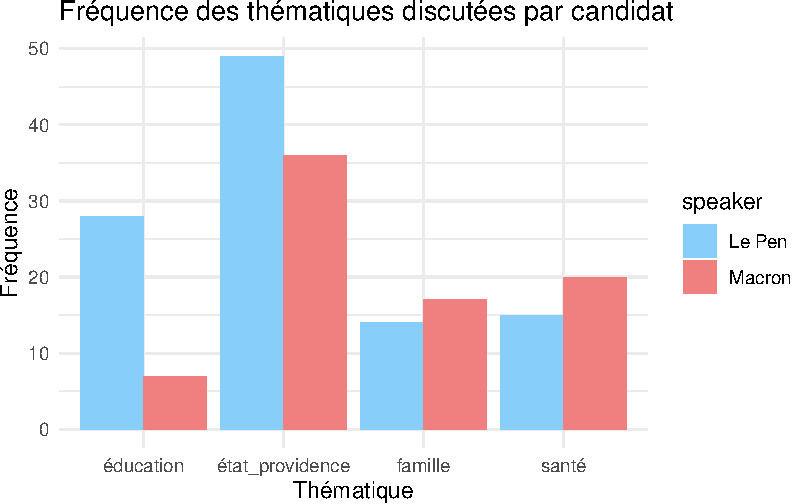
\includegraphics{tp3-fas1001-Saffioti_files/figure-pdf/unnamed-chunk-2-1.pdf}

}

\end{figure}



\end{document}
